\documentclass[12pt, times news roman, a4paper] {article}
\usepackage{graphicx}
\usepackage{caption}
\renewcommand{\figurename} {penjelasan}
\begin{document}
\begin{center}
\large{Resume seminar Oracle}\\

\noindent Muh Amri Irianto (1184100)

\end{center}

\begin {enumerate}
\section{Pembahasan}
\item pengembangan aplikasi rendah
\item Aplikasih Oracle express
\item Mengkonnversih spreadshett ke apliasih web dalam hitungan menit-demo aplikasi 
\item Oracle Apex Pendidikan
\item Laboratorium Tangan
\end{enumerate}

\begin{enumerate}
\section{Apa itu Kode Rendah?}
\item Mudah Dijalankan
\item sangat produktif
\item Scalable
\item Dapat Diperpanjang
\item kaya secara fungsional dengan kode lebih sedikit
\end{enumerate}

\begin {enumerate}
\section{Mengelola Data Dalam Spreadsheet}
\item  Memvalidasi Data Secara Manual Dan Rawan Kesalahan
\item  Integrase Data -Tidak Dapat Menjamin Keakuratan Data 	Di Lingkungan Multi-Pengguna.
\item  Penguncian Sel Keamanan Data Tidak Efektif.
\item  Berbagi Data-Excel Lamban Dan Sulit Untuk Dibagikan
\item  Puncak Oracle
\end{enumerate}

\section{pengaplikasian}
	\begin{minipage}{\linewidth}
		\centering
			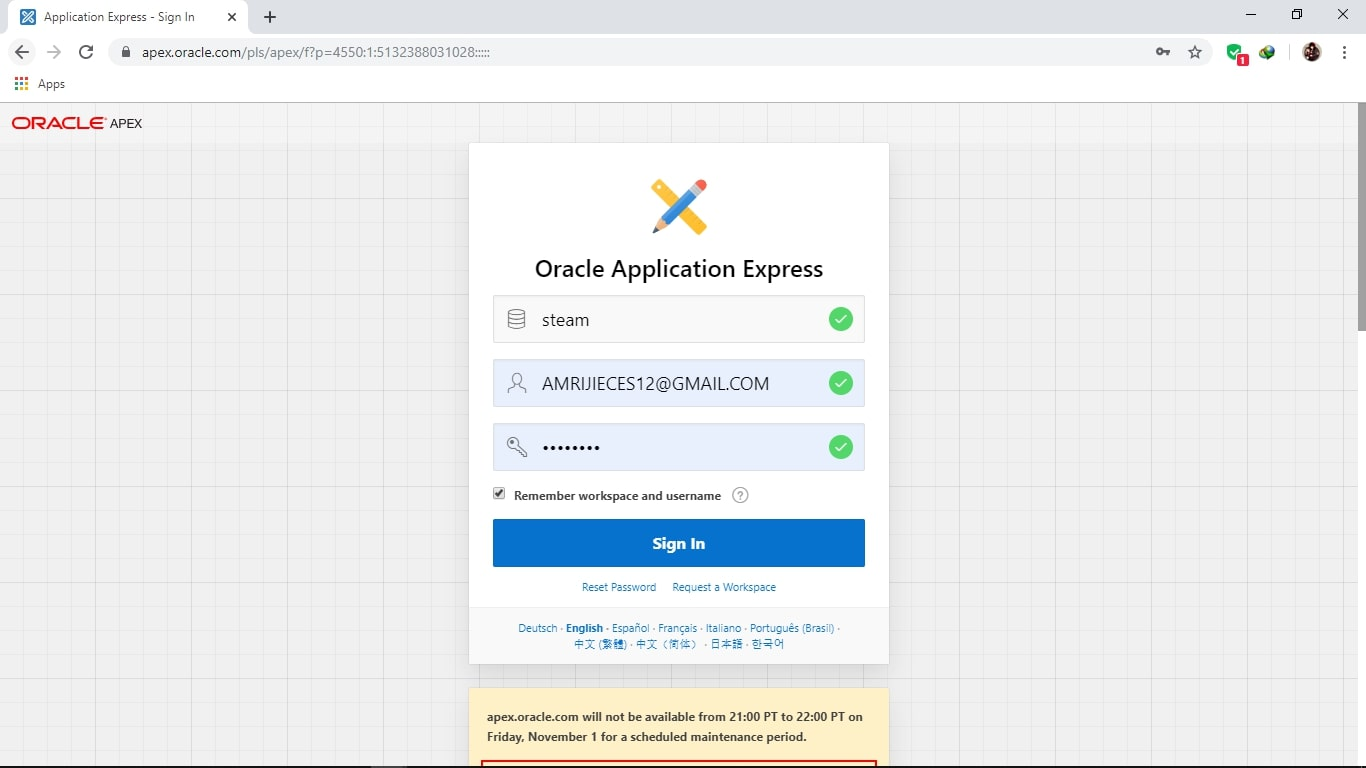
\includegraphics[width=12cm]{Capture1.jpg} 
			\captionof{figure} {masuk ke situs oracle}
	\end{minipage}

	\begin{minipage}{\linewidth}
	\centering
	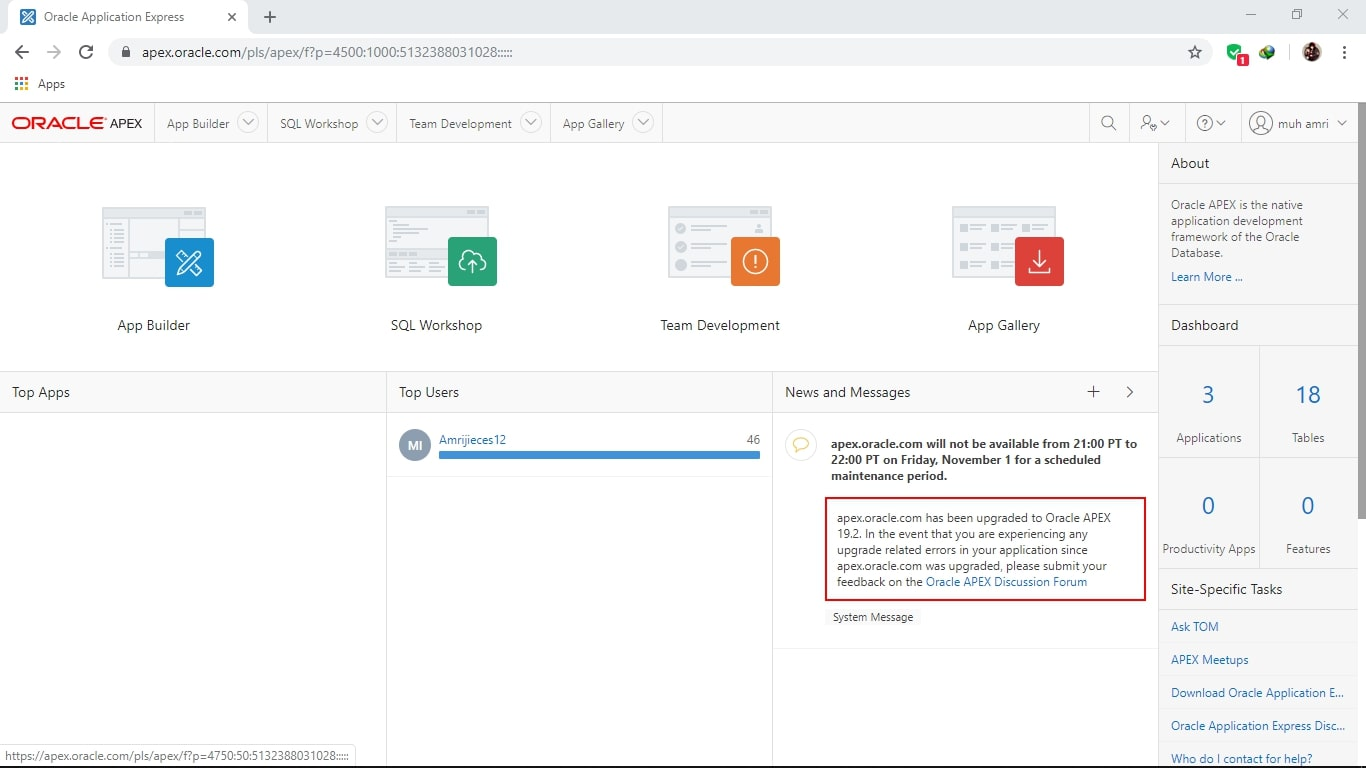
\includegraphics[width=12cm]{Capture2.jpg} 
	\captionof{figure} {Klik APP Builder}
\end{minipage}

	\begin{minipage}{\linewidth}
	\centering
	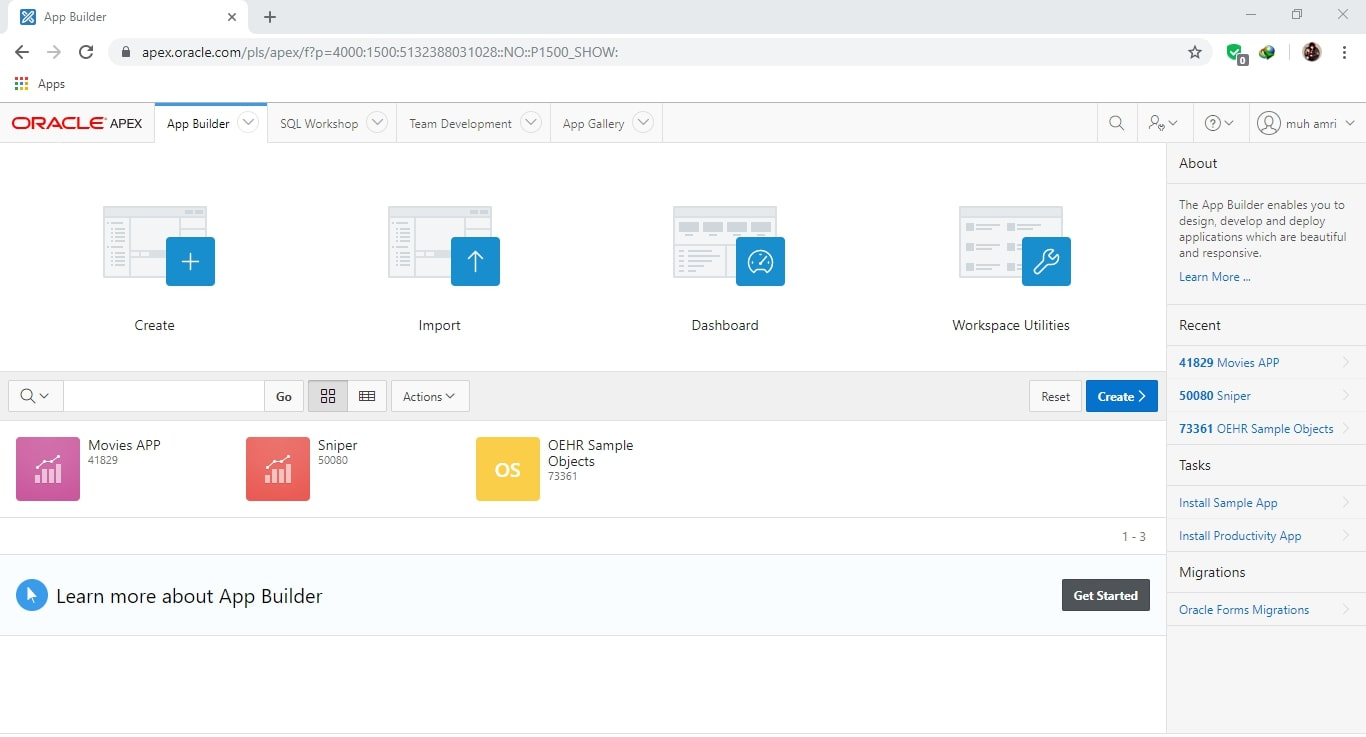
\includegraphics[width=12cm]{Capture3.jpg} 
	\captionof{figure} {Tekan Tombol Create}
\end{minipage}

	\begin{minipage}{\linewidth}
	\centering
	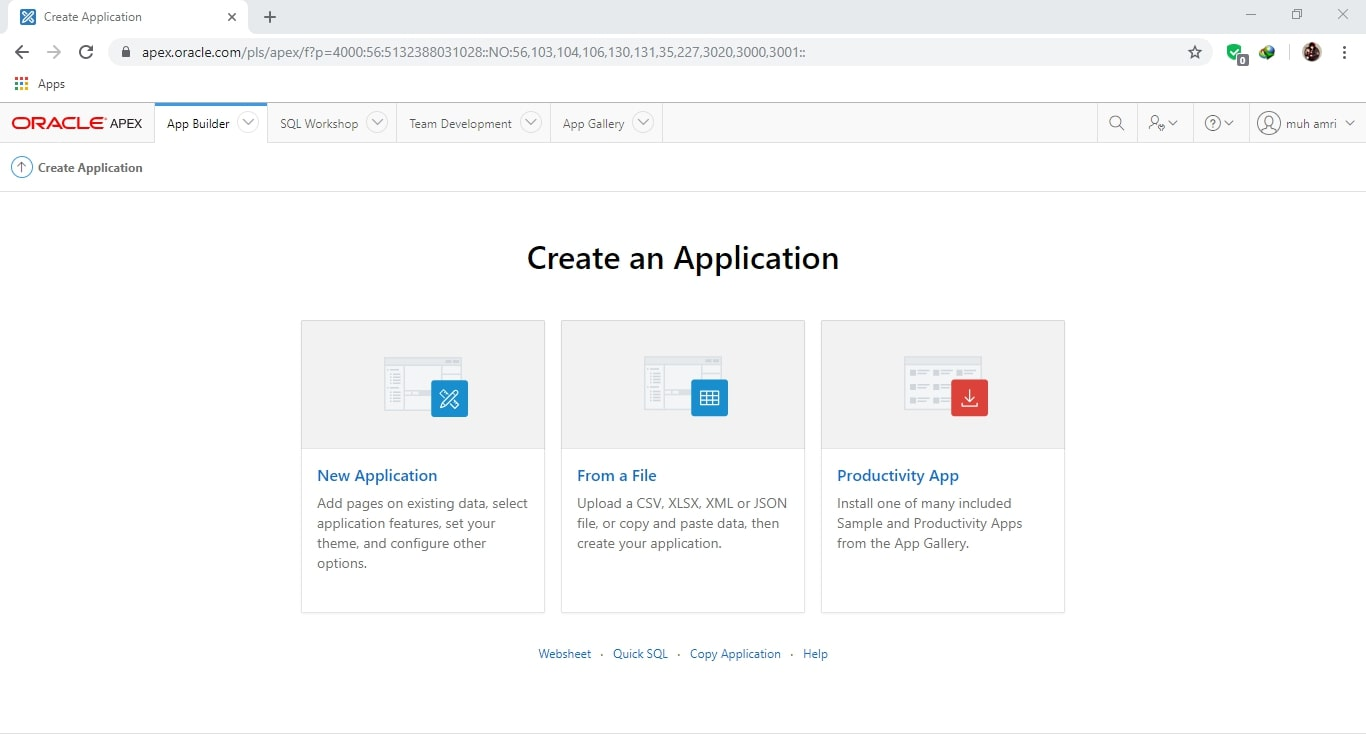
\includegraphics[width=12cm]{Capture4.jpg} 
	\captionof{figure} {Kita akan diarah menuju 3 pilihan pada pilihan ini kita akan tekan di tengan yaitu "From A File"}
\end{minipage}

	\begin{minipage}{\linewidth}
	\centering
	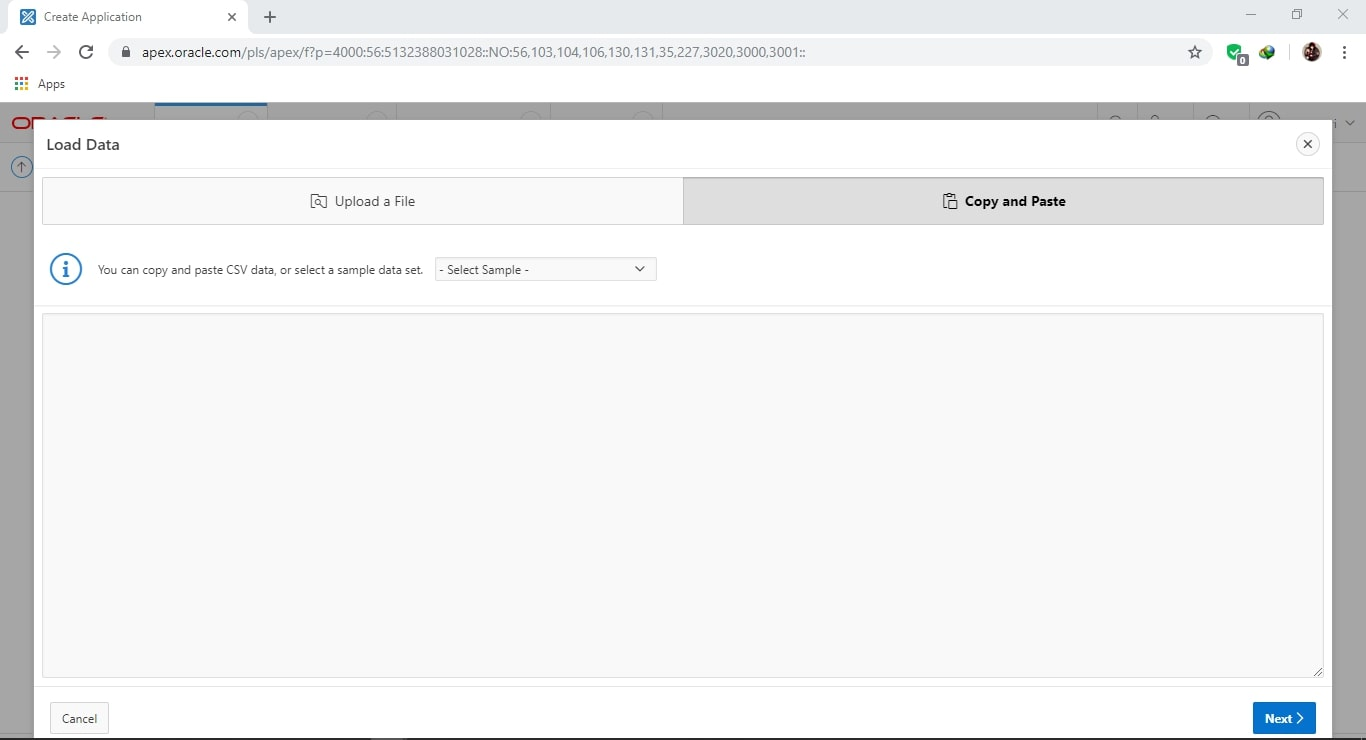
\includegraphics[width=12cm]{Capture5.jpg} 
	\captionof{figure} {Setelah Ituh Pilih Copy Paste Untuk mencoba file yang telah disediakan}
\end{minipage}

	\begin{minipage}{\linewidth}
	\centering
	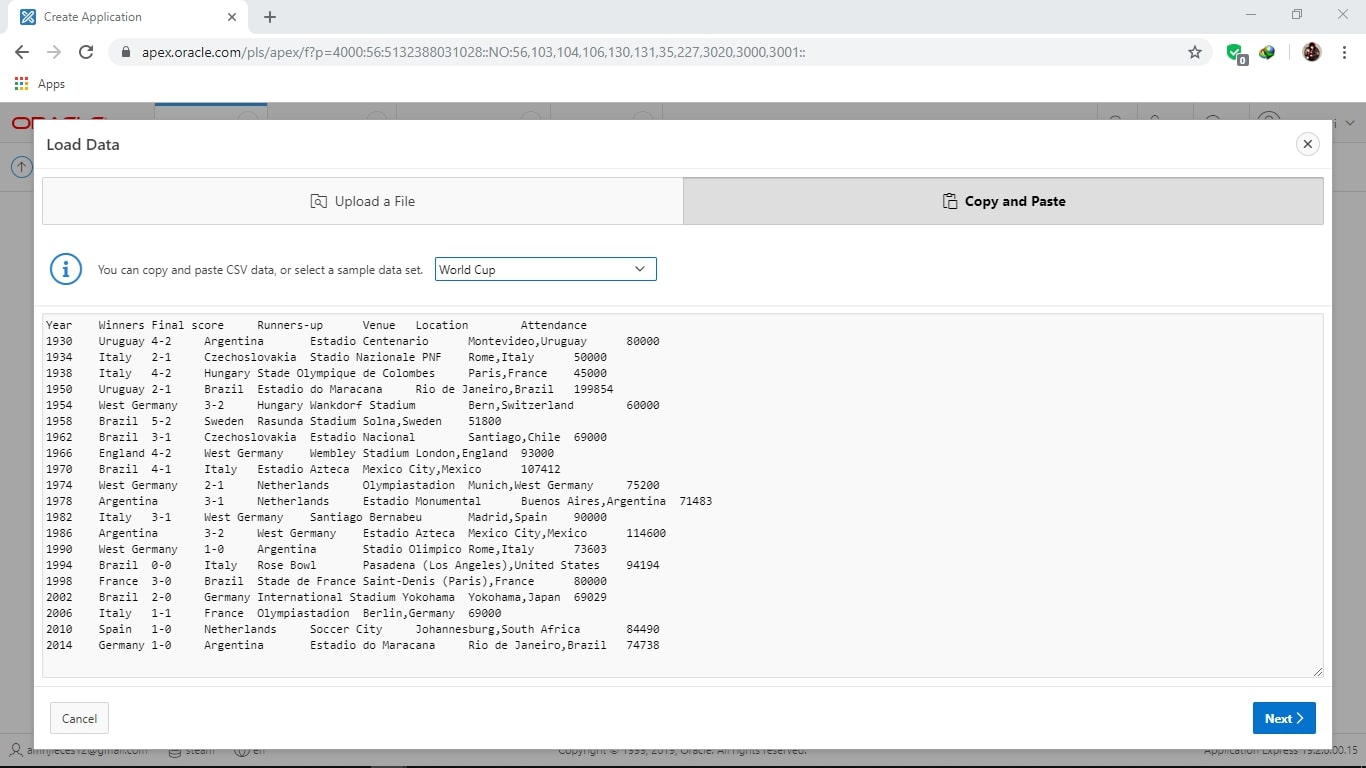
\includegraphics[width=12cm]{Capture6.jpg} 
	\captionof{figure} {Kita Pilih"world cup" }
\end{minipage}

	\begin{minipage}{\linewidth}
	\centering
	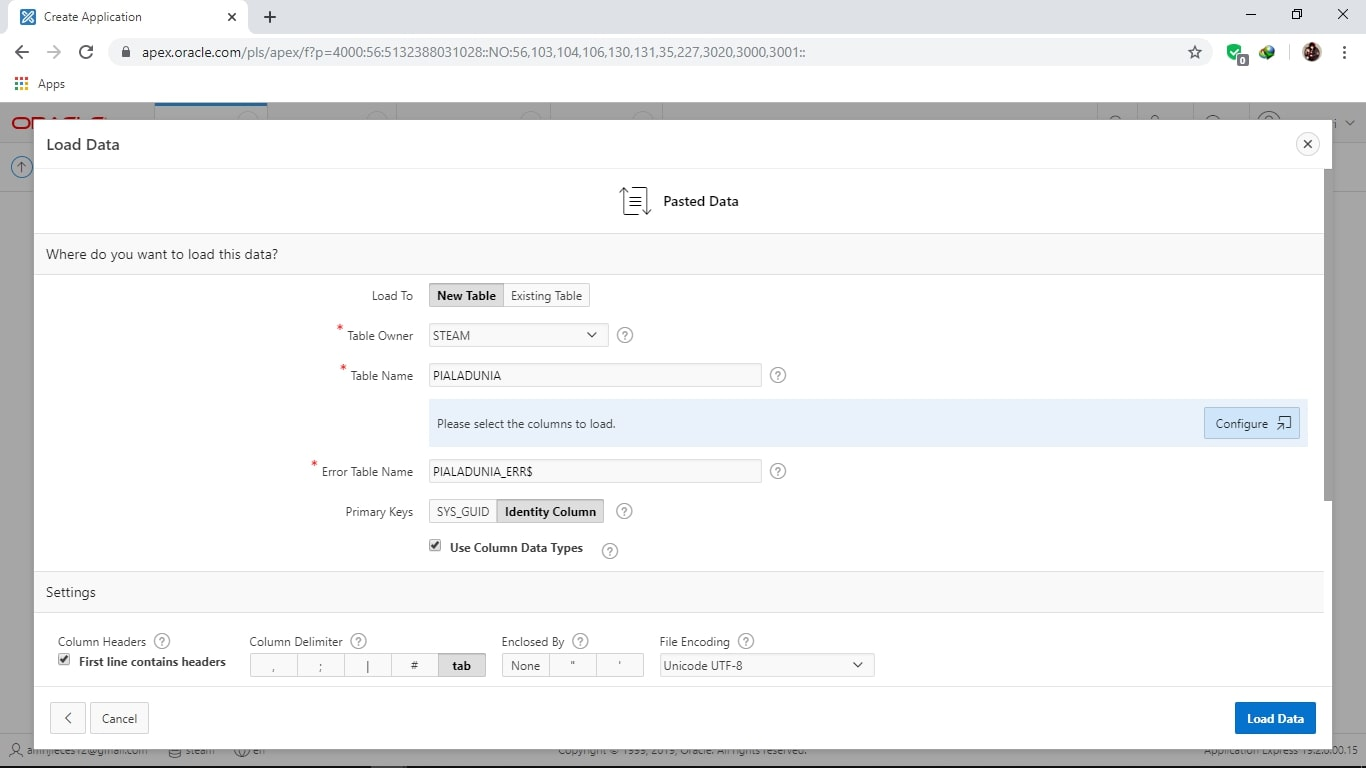
\includegraphics[width=12cm]{Capture7.jpg} 
	\captionof{figure} {Kita bisa mengganti nama app yang akan kita buat tekan "load data"}
\end{minipage}

	\begin{minipage}{\linewidth}
	\centering
	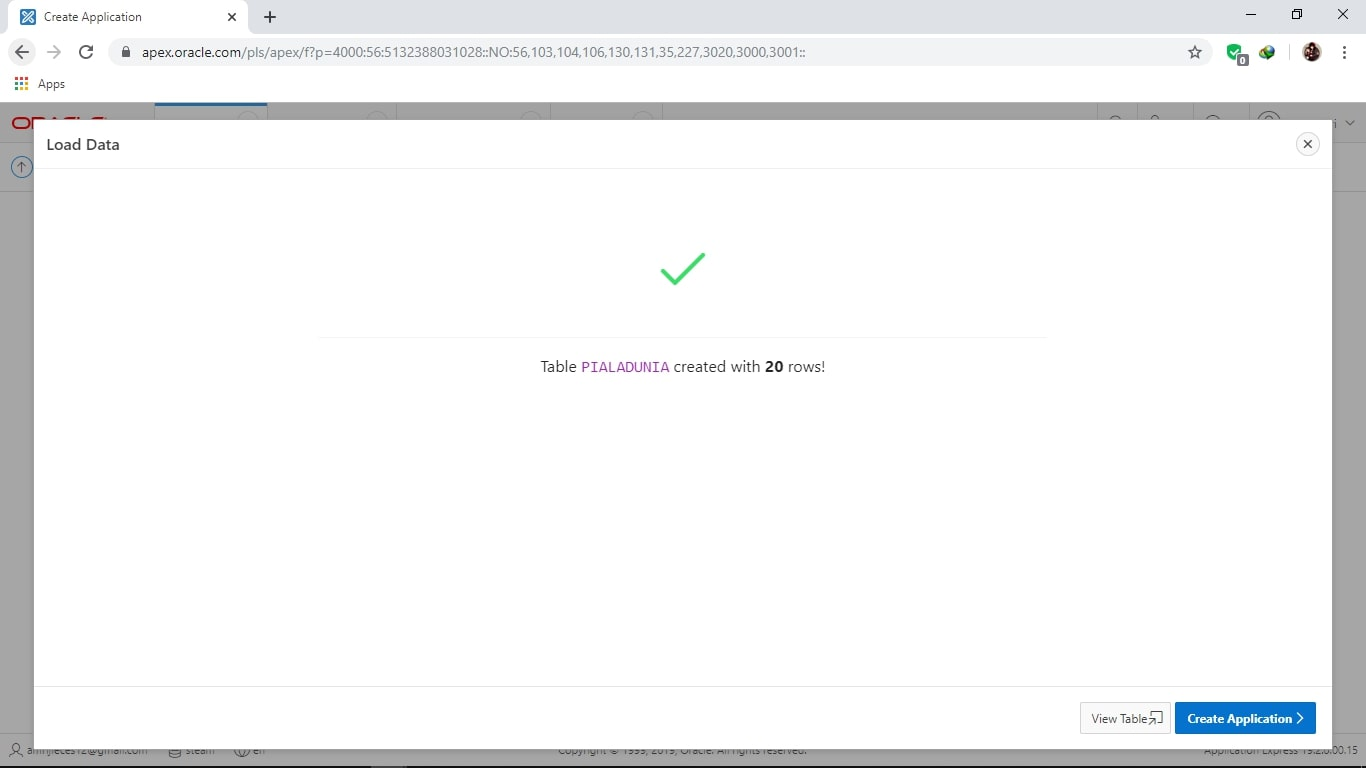
\includegraphics[width=12cm]{Capture9.jpg} 
	\captionof{figure} {Ketika selesai kita pilih "create aplication"}
\end{minipage}

	\begin{minipage}{\linewidth}
	\centering
	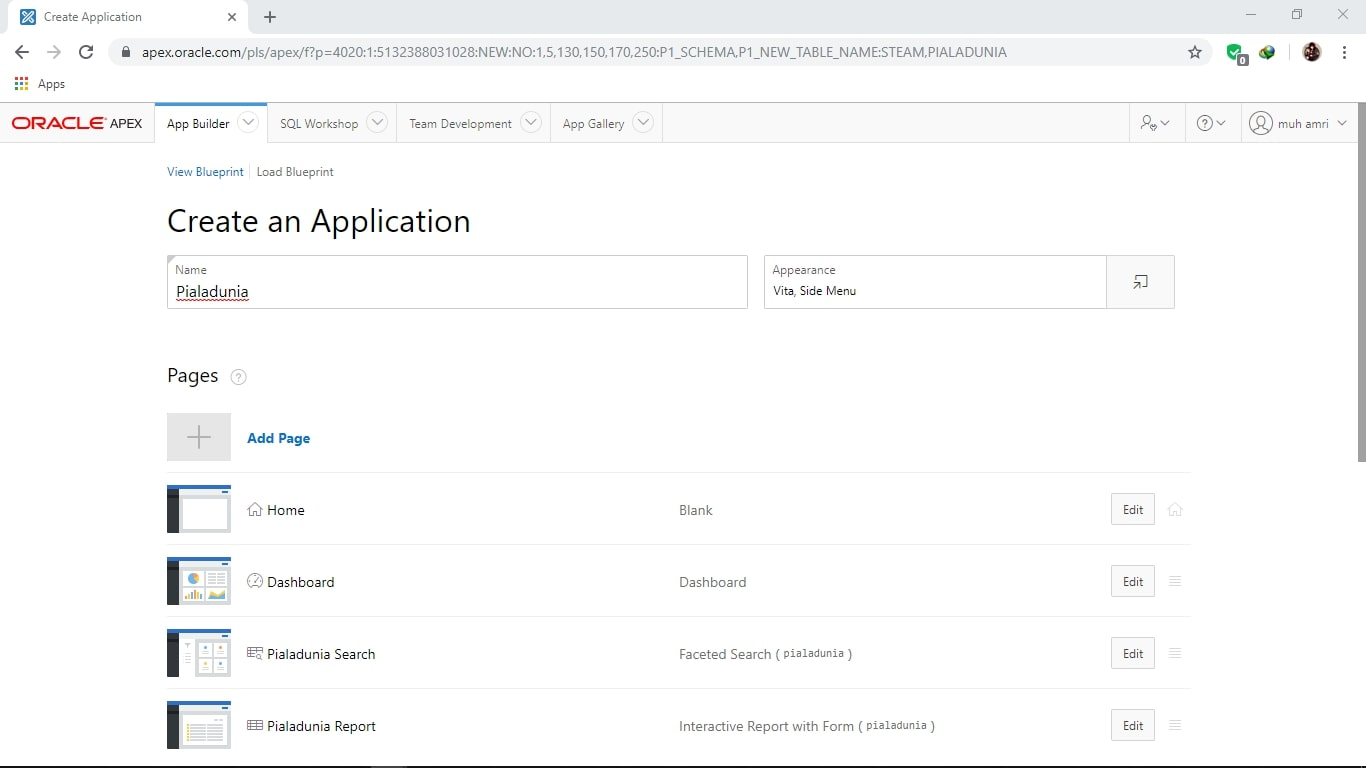
\includegraphics[width=12cm]{Capture10.jpg} 
	\captionof{figure} {kita mulai dengan custominasi pada app yang akan kita buat}
\end{minipage}

	\begin{minipage}{\linewidth}
	\centering
	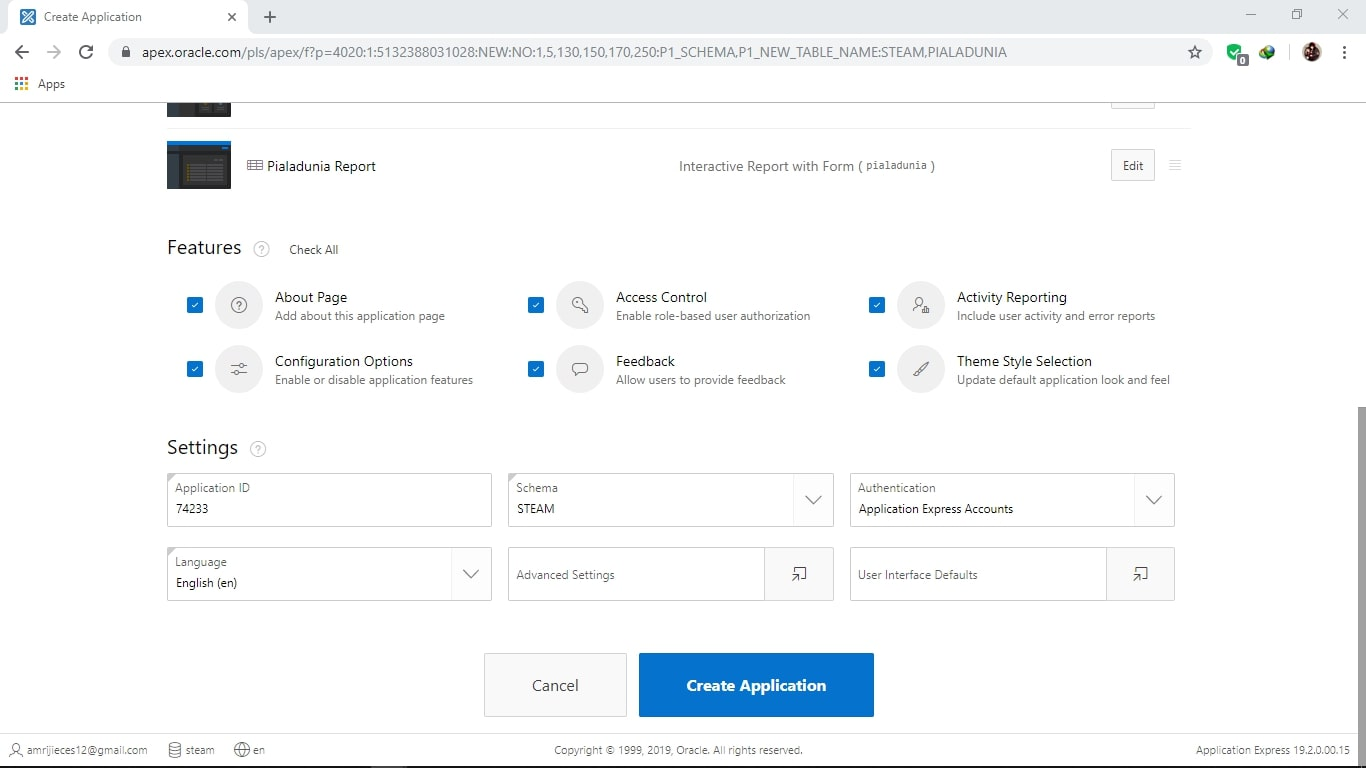
\includegraphics[width=12cm]{Capture11.jpg} 
	\captionof{figure} {geser yang paling bawah tekan create aplication}
\end{minipage}

	\begin{minipage}{\linewidth}
	\centering
	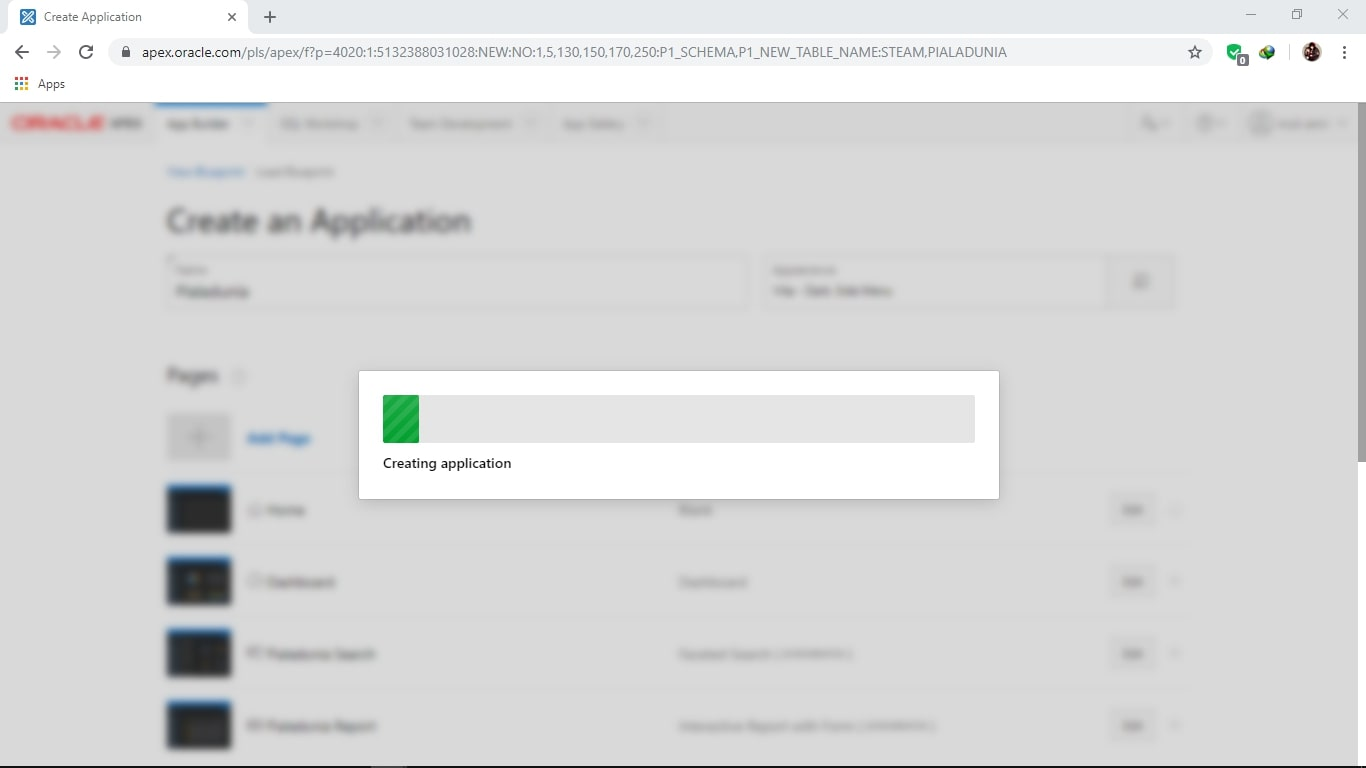
\includegraphics[width=12cm]{Capture12.jpg} 
	\captionof{figure} {tunggu proses hingga selesai}
\end{minipage}

\begin{minipage}{\linewidth}
	\centering
	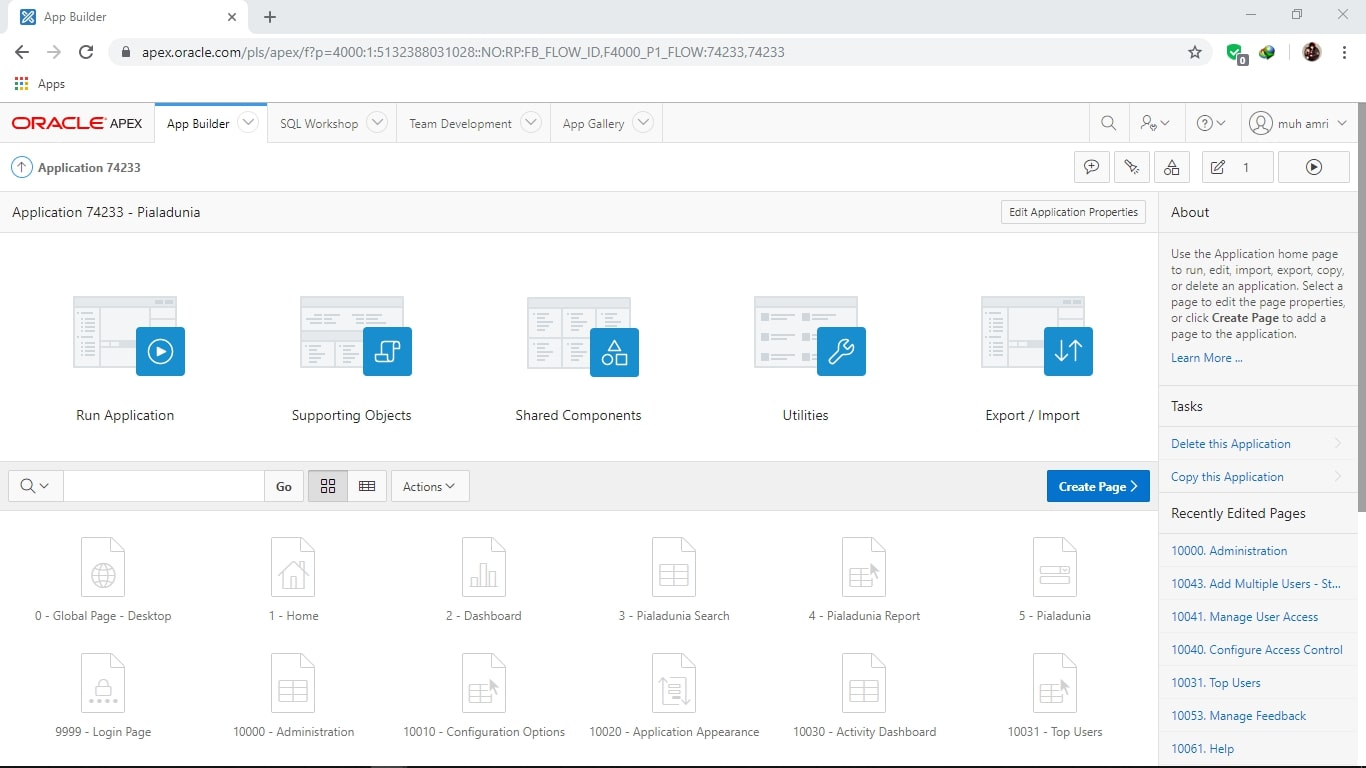
\includegraphics[width=12cm]{Capture13.jpg} 
	\captionof{figure} {applikasi data worldcup siap}
\end{minipage}

\begin {enumerate}
\section{Apa Itu Oracle Apex?}
\item  Mengembangkan Aplikasi Web Desktop Dan Seluler
\item  Memvisualisasikan Dan Memelihara Data Basis Data,
\item  Meningkatkan Keterampilan Sql Dan Kemampuan Basis Data.
Oracle Apex: Use Cases
\end{enumerate}

\section {aplikasi sederhana APEX}
\begin{minipage}{\linewidth}
	\centering
	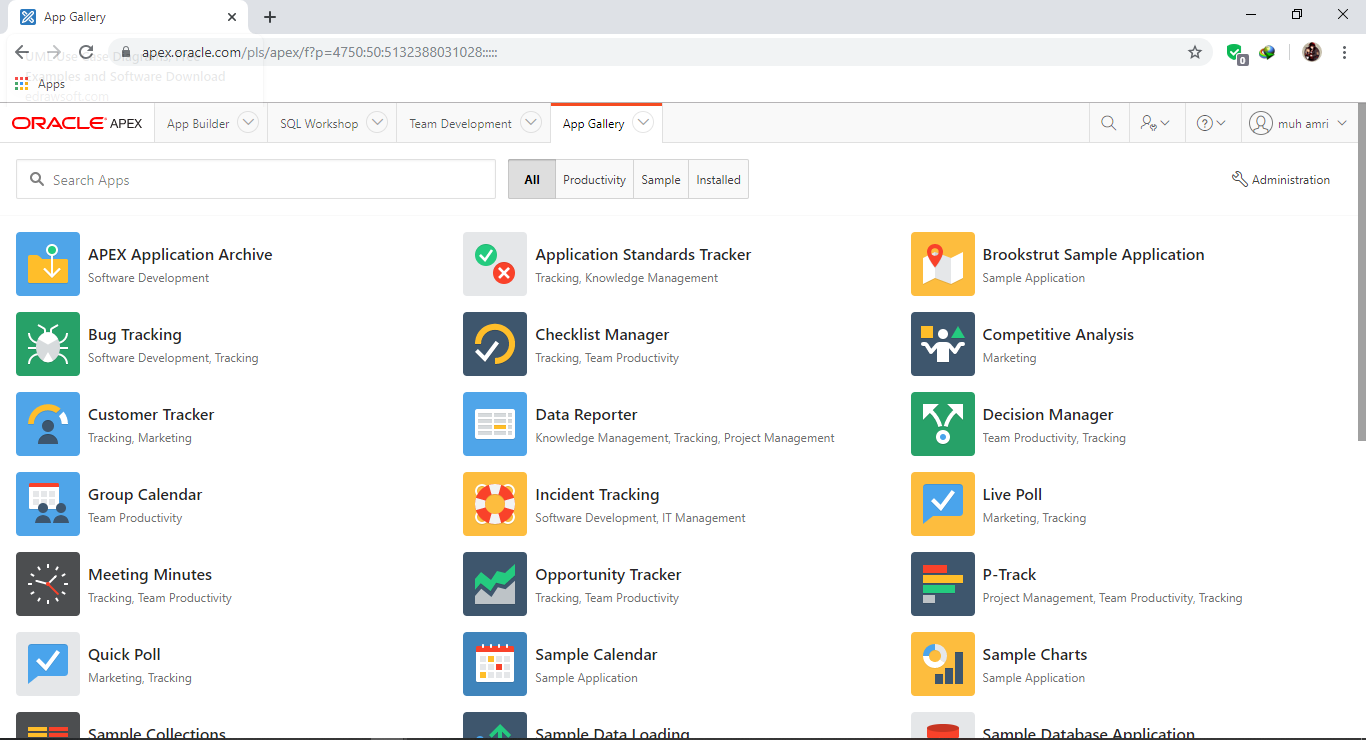
\includegraphics[width=12cm]{Gambar.png} 
	\captionof{figure} {kita masuk ke sample app}
\end{minipage}

\begin{minipage}{\linewidth}
	\centering
	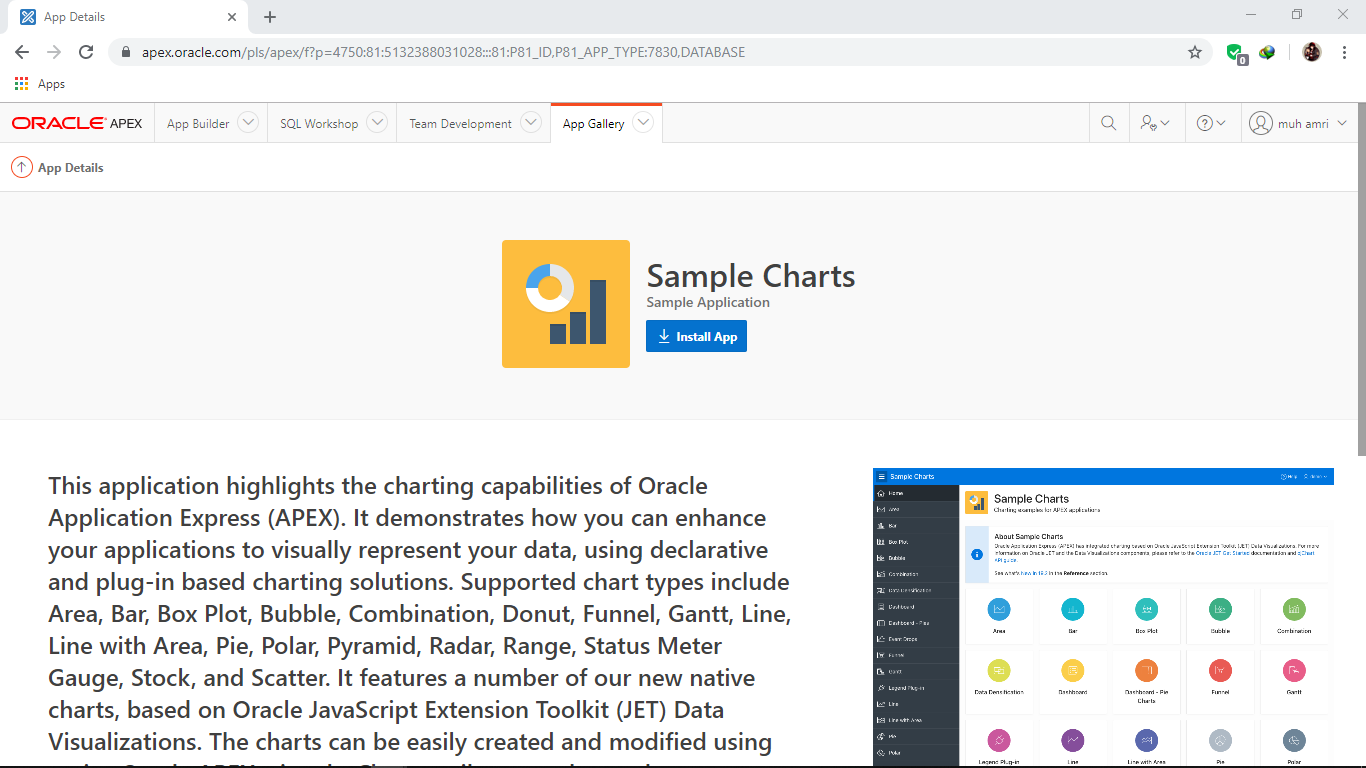
\includegraphics[width=12cm]{Gambar2.png} 
	\captionof{figure} {Kita pilih aplikasi yang akan dimasukkan}
\end{minipage}\\
\\
\begin{minipage}{\linewidth}
	\centering
	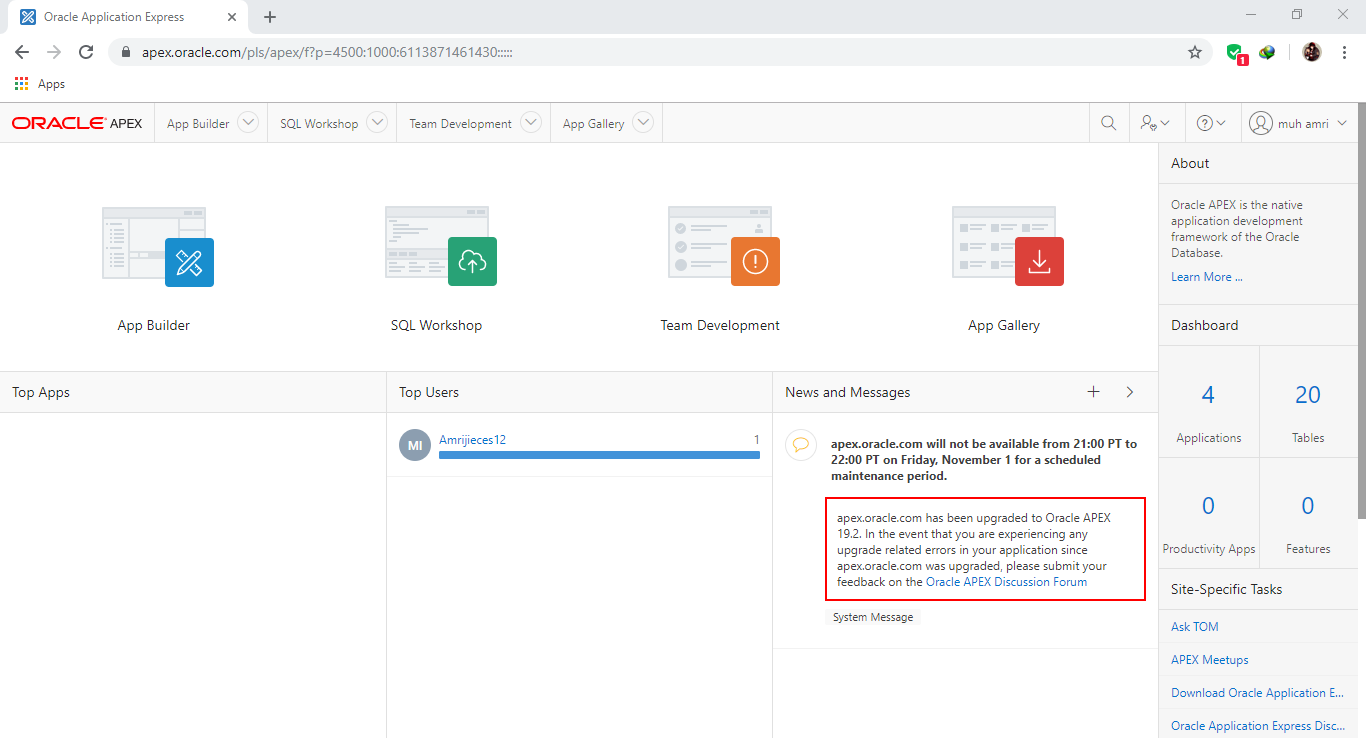
\includegraphics[width=12cm]{Gambar3.png} 
	\captionof{figure} {terus klik next dan klik instal}
\end{minipage}\\
\\
\begin{minipage}{\linewidth}
	\centering
	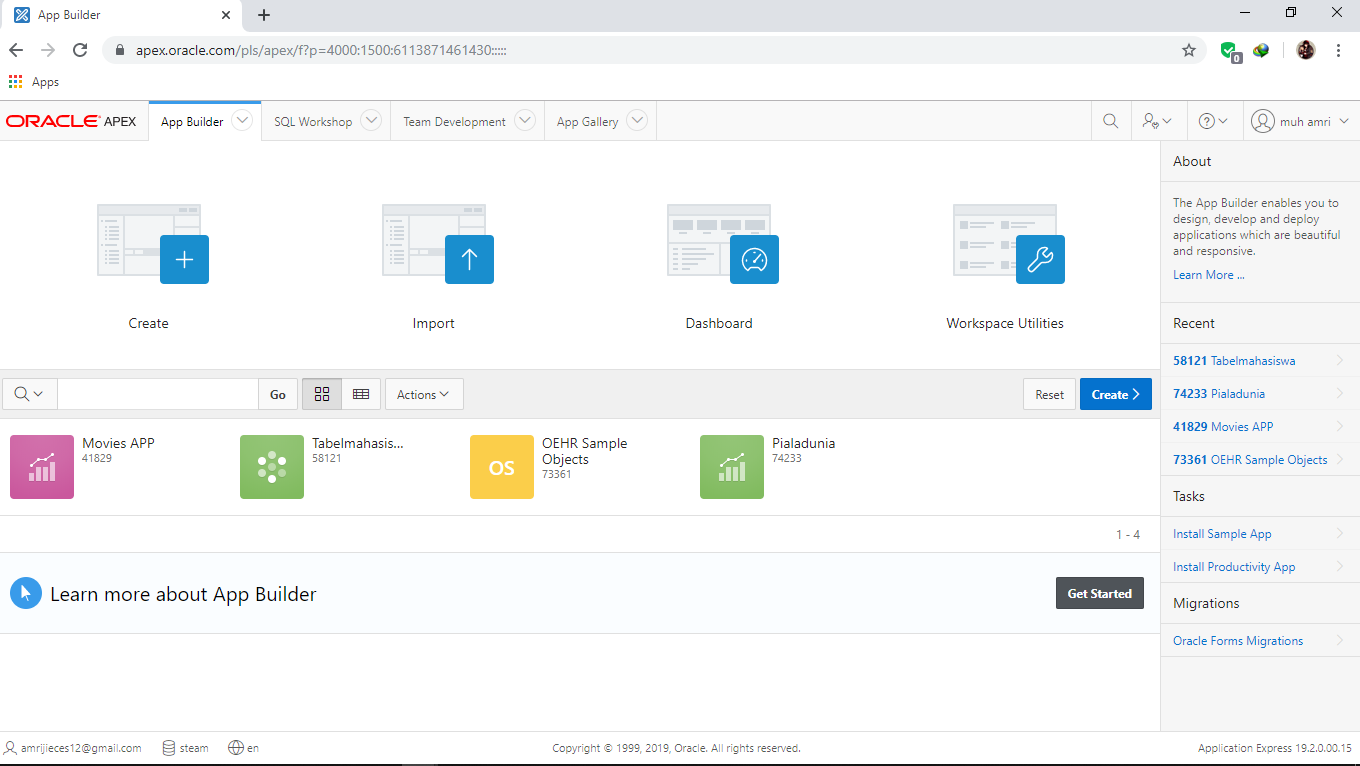
\includegraphics[width=12cm]{Gambar4.png} 
	\captionof{figure} {kalau sudah maka gambar akan terwujud seperti yang diatas}
\end{minipage}\\
\\
\begin{minipage}{\linewidth}
	\centering
	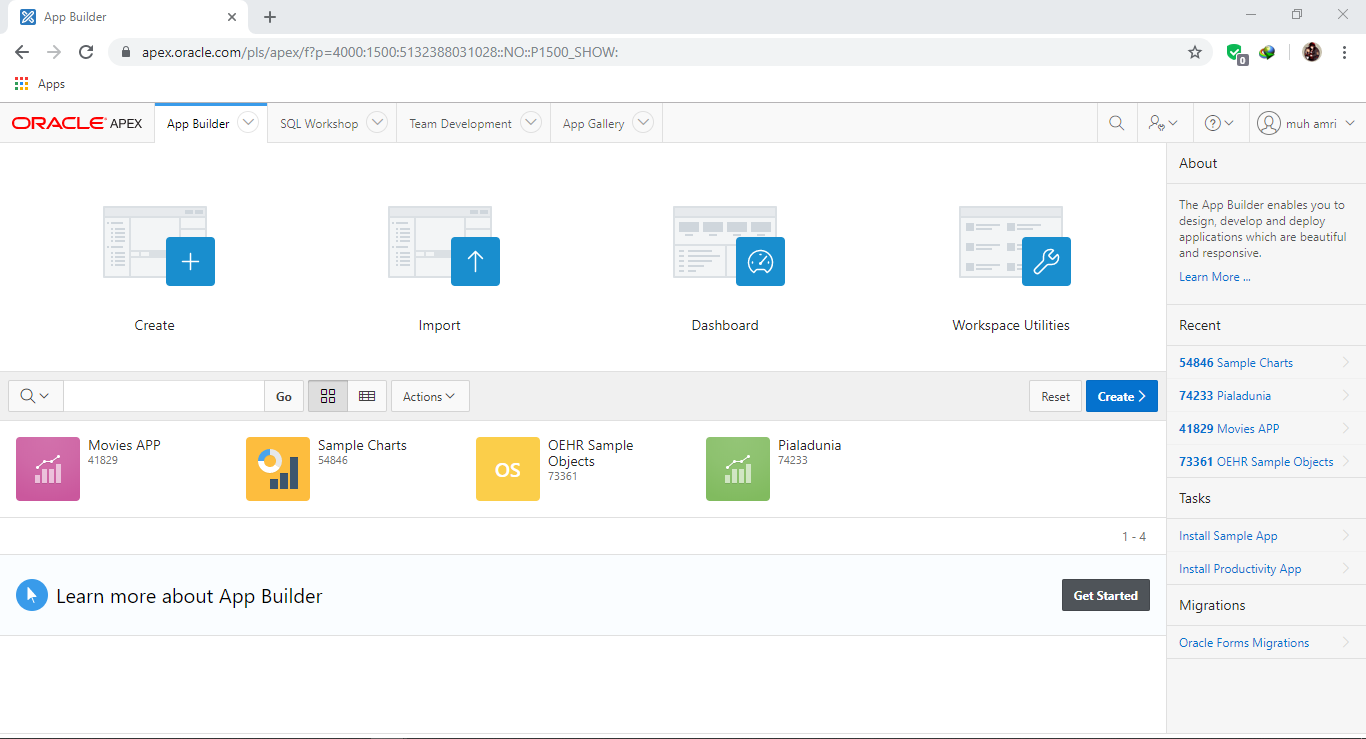
\includegraphics[width=12cm]{Gambar5.png} 
	\captionof{figure} {kita bisa run saat kita memasuki app builder}
\end{minipage}
\end{document}